\documentclass[12pt,a4paper]{report}
\usepackage[utf8]{vietnam}
\usepackage{amsmath}
\usepackage{amsfonts}
\usepackage{amssymb}
\usepackage{makeidx}
\usepackage{graphicx}
\usepackage{fancybox}
\usepackage{boxedminipage}
\usepackage{multirow}
\usepackage[left=3.50cm, right=2.00cm, top=3.50cm, bottom=3.00cm]{geometry}
\usepackage{scrextend}
\changefontsizes{13pt}
\begin{document}
	\thisfancypage{%đóng khung trang này
		\setlength{\fboxsep}{0pt}% 8pt là độ dày của đường viền
		\fbox}{} % phần nội dung sau là tương tự như đã làm
	\thispagestyle{empty}
	\begin{center}
		\vspace*{0.2cm}
		\fontsize{14}{12}
		\textbf{TRƯỜNG ĐẠI HỌC BÁCH KHOA HÀ NỘI}\\
		\textbf{VIỆN TOÁN ỨNG DỤNG VÀ TIN HỌC}\\
		\textbf{------ o0o ------}
	\end{center}
	\vspace*{0.8cm}
	\begin{center}
		
\includegraphics[scale=.5]{bk.png}
	\end{center}
	\vspace*{0.8cm}
	\begin{center}
		\fontsize{20}{18}
		\textbf{BÁO CÁO MÔN HỌC\\ CƠ SỞ DỮ LIỆU NÂNG CAO}\\
		\vspace*{0.8cm}
		\fontsize{18}{16}
	\end{center}
	\vspace*{0.7cm}
	\begin{center}
		\fontsize{14}{16}
		\begin{tabular}{ll}
			 
			\textbf{Sinh viên thực hiện:} & \textbf{Hoàng Thanh Lưu} \\ 
			\textbf{Mã số sinh viên:} & \textbf{20162602}\\
			\textbf{Lớp:}  & \textbf{Toán Tin K61} \\ 
		\end{tabular} \\
		\vspace*{2.5cm}
		\fontsize{14}{16}
		\textbf{Hà Nội - 6/2020}
	\end{center}

	\chapter*{Lời nói đầu}
	Ngày nay, trong xu thế phát triển không ngừng của công nghệ thông tin, đặc biệt trong giai đoạn Cách mạng công nghiệp 4.0, các công ty, doanh nghiệp đặc biệt quan tâm tới dữ liệu. Khối lượng dữ liệu cần xử lý và phân tích dần dần tích lũy nhiều hơn đòi hỏi ngành khoa học nghiên cứu dữ liệu lớn ra đời. Cùng với đó, các cộng nghệ về khai phá dữ liệu lớn, các hệ quản trị cơ sở dữ liệu được đưa ra nhằm giải quyết các vấn đề về dữ liệu, dần trở thành nhu cầu thiết yếu của nghiên cứu khoa học và xã hội. Một trong số hệ quản trị cơ sở dữ liệu nổi lên đó có thể kể đến như Oracle, SQL Server, …\\\\
	Môn học \textit{“Cơ sở dữ liệu nâng cao”} đã cung cấp các kiến thức liên quan đến việc phân tích, xử lý, xây dựng một hệ cơ sở dữ liệu, các vấn đề xử lý tương tranh các giao tác, nghiên cứu cơ sở dữ liệu phân tán và cơ sở dữ liệu song song, dữ liệu lớn – Big Data, kho dữ liệu – Data warehouse, … Nghiên cứu về hệ quản trị cơ sở dữ liệu Oracle,…\\\\
	Em xin gửi lời cảm ơn chân thành nhất tới các thầy cô phụ trách học phần: \textit{TS.Nguyễn Thị Thanh Huyền}, \textit{ThS Nguyễn Tuấn Dũng} và \textit{ThS Nguyễn Danh Tú} đã hướng dẫn, chỉ bảo và tạo điều kiện giúp em có thể hoàn thành học phần và báo cáo môn học. Do thời gian, kiến thức và kinh nghiệm còn nhiều hạn chế nên báo cáo còn nhiều thiếu sót, vì vậy em rất mong nhận được những ý kiến góp ý của thầy cô để báo cáo có thể hoàn thiện hơn.\\\\
	Em xin chân thành cảm ơn!
	\tableofcontents
	\chapter{Cơ sở dữ liệu lớn}
	\section{Thế nào là cơ sở dữ liệu lớn?}
	Theo [3], Big Data là một trong 4 xu hướng công nghệ hiện nay, bao gồm: Dữ liệu lớn (\textit{Big Data}), Đám mây (\textit{Cloud}), Mạng xã hội (\textit{Social Networks}) và Di động (\textit{Mobulity}). \\\\
	Theo Wikipedia, Dữ liệu lớn (Tiếng Anh: Big data) là một thuật ngữ cho việc xử lý một tập hợp dữ liệu rất lớn và phức tạp mà các ứng dụng xử lý dữ liệu truyền thống không xử lý được. Dữ liệu lớn bao gồm các thách thức như phân tích, thu thập, giám sát dữ liệu, tìm kiếm, chia sẻ, lưu trữ, truyền nhận, trực quan, truy vấn và tính riêng tư. Thuật ngữ này thường chỉ đơn giản đề cập đến việc sử dụng các phân tích dự báo, phân tích hành vi người dùng, hoặc một số phương pháp phân tích dữ liệu tiên tiến khác trích xuất giá trị từ dữ liệu mà ít khi đề cập đến kích thước của bộ dữ liệu.\\\\
	Dữ liệu lớn thường bao gồm tập hợp dữ liệu với kích thước vượt xa khả năng của các công cụ phần mềm thông thường để thu thập, hiển thị, quản lý và xử lý dữ liệu trong một thời gian có thể chấp nhận được. Kích thước dữ liệu lớn là một mục tiêu liên tục thay đổi. Như năm 2012 thì phạm vi một vài tá terabytes tới nhiều petabytes dữ liệu. Dữ liệu lớn yêu cầu một tập các kỹ thuật và công nghệ được tích hợp theo hình thức mới để khai phá từ tập dữ liệu đa dạng, phức tạp, và có quy mô lớn.
	\begin{figure}[h]
		\centering
		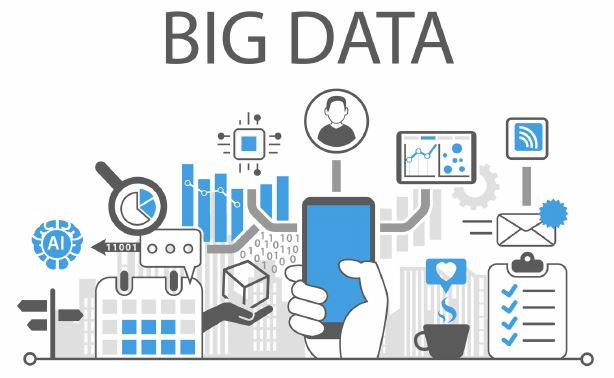
\includegraphics[scale=.7]{b-1-1.jpg}
		\caption{Cơ sở dữ liệu lớn - BigData}
	\end{figure}
	\section{Đặc trưng cơ bản của cơ sở dữ liệu lớn}
	Big Data được mô tả bởi những đặc trưng sau:
	\subsection{Dung lượng (Volume)}
	Đây là đặc điểm tiêu biểu nhất của dữ liệu lớn, khối lượng dữ liệu rất lớn. Kích cỡ của Big data đang từng ngày tăng lên, và tính đến năm 2012 thì nó có thể nằm trong khoảng vài chục terabyte cho đến nhiều petabyte (1 petabyte = 1024 terabyte) chỉ cho một tập hợp dữ liệu. Dữ liệu truyền thống có thể lưu trữ trên các thiết bị đĩa mềm, đĩa cứng. Nhưng với dữ liệu lớn chúng ta sẽ sử dụng công nghệ đám mây mới đáp ứng khả năng lưu trữ được dữ liệu lớn.
	\subsection{Tốc độ (Velocity)}
	Tốc độ có thể hiểu theo 2 khía cạnh:
	\begin{itemize}
		\item[\textbf{(a)}] Khối lượng dữ liệu gia tăng rất nhanh (mỗi giây có tới 72.9 triệu các yêu cầu truy cập tìm kiếm trên web bán hàng của Amazon); \item[\textbf{(b)}] Xử lý dữ liệu nhanh ở mức thời gian thực (real-time), có nghĩa dữ liệu được xử lý ngay tức thời ngay sau khi chúng phát sinh (tính đến bằng mili giây). Các ứng dụng phổ biến trên lĩnh vực Internet, Tài chính, Ngân hàng, Hàng không, Quân sự, Y tế- Sức khỏe như hiện nay phần lớn dữ liệu lớn được xử lý real-time. Công nghệ xửxử lý dữ liệu lớn ngày nay đã cho phép chúng ta xử lý tức thì trước khi được lưu trữ vào cơ sở dữ liệu.
		
	\end{itemize} \subsection{Đa dạng (Variety)}
	Đối với dữ liệu truyền thống chúng ta hay nói đến dữ liệu có cấu 
	trúc, thì ngày nay hơn 80\% dữ liệu được sinh ra là phi cấu trúc (tài liệu, blog, hình ảnh, video, bài hát, dữ liệu từ thiết bị cảm biến vật lý, thiết bị chăm sóc sức khỏe $\cdots$). Big data cho phép liên kết và phân tích nhiều dạng dữ liệu khác nhau. Ví dụ, với các bình luận của một nhóm người dùng nào đó trên Facebook với thông tin video được chia sẻ.
	\begin{figure}[h]
		\centering
		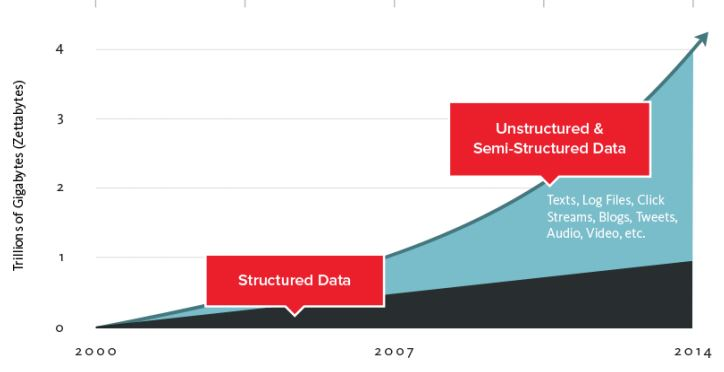
\includegraphics[scale=.6]{b-2.jpg}
		\caption{Hơn 80\% dữ liệu là phi cấu trúc}
	\end{figure}
	\subsection{Độ tin cậy (Veracity)}
	Một trong những tính chất phức tạp nhất của Dữ liệu lớn là độ tin cậy/chính xác của dữ liệu. Với xu hướng phương tiện truyền thông xã hội (Social Media) và mạng xã hội (Social Network) ngày nay và sự gia tăng mạnh mẽ tính tương tác và chia sẻ của người dùng Mobile làm cho bức tranh xác định về độ tin cậy và chính xác của dữ liệu ngày một khó khăn hơn. Bài toán phân tích và loại bỏ dữ liệu thiếu chính xác và nhiều đang là tính chất quan trọng của Big data.
	\subsection{Giá trị (Value)}
	Giá trị là đặc điểm quan trọng nhất của dữ liệu lớn, vì khi bắt đầu triển khai xây dựng dữ liệu lớn thì việc đầu tiên chúng ta cần phải làm đó là xác định được giá trị của thông tin mang lại như thế nào, khi đó chúng ta mới có quyết định có nên triển khai dữ liệu lớn hay không. Nếu chúng ta có dữ liệu lớn mà chỉ nhận được 1\% lợi ích từ nó, thì không nên đầu tư phát triển dữ liệu lớn. Kết quả dự báo chính xác thể hiện rõ nét nhất về giá trị của dữ liệu lớn mang lại. Ví dụ, từ khối dữ liệu phát sinh trong quá trình khám, chữa bệnh sẽ giúp dự báo về sức khỏe được chính xác hơn, sẽ giảm được chi phí điều trị và các chi phí liên quan đến y tế. 
	\begin{figure}[h]
		\centering
		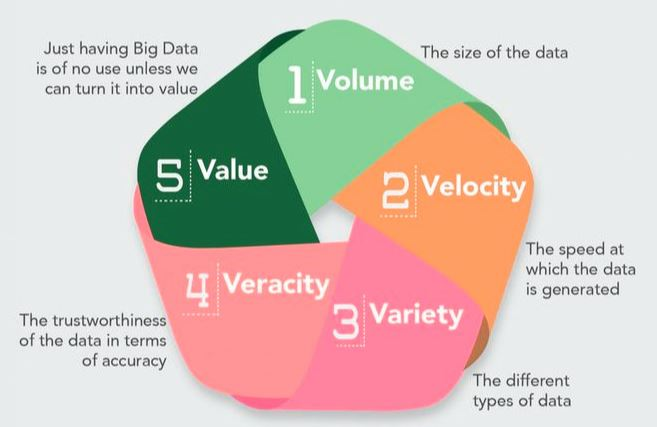
\includegraphics[scale=.6]{b-3.jpg}
		\caption{Đặc trưng của Big data}
	\end{figure}
\section{Các ứng dụng của cơ sở dữ liệu lớn}
\subsection{Quản lý chính phủ}
Việc sử dụng các dữ liệu lớn trong các quy trình của chính phủ cho phép tăng hiệu quả về mặt chi phí, năng suất và sự đổi mới, nhưng không phải là không có sai sót của nó. Phân tích dữ liệu thường yêu cầu nhiều bộ phận của chính phủ (trung ương và địa phương) hợp tác và tạo ra các quy trình mới và sáng tạo để mang lại kết quả mong muốn. 
\subsection{Sự phát triển quốc tế}
Nghiên cứu về việc sử dụng hiệu quả các công nghệ thông tin và truyền thông cho mục đích phát triển (hay còn gọi là ICT4D) cho thấy công nghệ dữ liệu lớn có thể có nhiều đóng góp quan trọng nhưng cũng là thách thức đối với sự phát triển của quốc tế. Những tiến bộ trong phân tích dữ liệu lớn giúp giảm chi phí cho việc ra quyết định trong các lĩnh vực quan trọng như chăm sóc sức khoẻ, việc làm, năng suất kinh tế, tội phạm, an ninh, thiên tai và quản lý tài nguyên. Tuy nhiên, những thách thức đối với các nước đang phát triển như cơ sở hạ tầng công nghệ không đầy đủ và sự khan hiếm về kinh tế và nguồn nhân lực sẽ làm nghiêm trọng thêm các mặt trái của dữ liệu lớn như sự riêng tư hoặc các vấn đề khác.
\subsection{Tài chính}
Việc sử dụng các dữ liệu lớn dưới dạng lịch sử các giao dịch tài chính được gọi là phân tích kỹ thuật. Sử dụng dữ liệu phi tài chính để dự đoán thị trường đôi khi được gọi là dữ liệu thay thế.
\subsection{Sản xuất}
Theo bài Nghiên cứu xu hướng toàn cầu TCS 2013, sự cải tiến trong kế hoạch sản xuất và chất lượng sản phẩm là lợi ích lớn nhất của dữ liệu lớn cho ngành sản xuất. Dữ liệu lớn cung cấp cơ sở hạ tầng cho ngành công nghiệp sản xuất, đó là khả năng cải thiện năng suất và tính khả dụng. Việc lên kế hoạch sản xuất chính là một cách tiếp cận dữ liệu lớn cho phép giảm thời gian chết về gần như bằng không và cụ thể hóa số lượng lớn dữ liệu và các công cụ dự đoán khác cho phép tạo ra một quá trình nhằm hệ thống hóa dữ liệu thành các thông tin hữu ích. Khái niệm về việc dự báo sản xuất bắt đầu bằng việc thu thập dữ liệu cảm quan khác nhau như âm thanh, chuyển động, áp suất, điện áp... Số lượng lớn các dữ liệu cảm quan cộng với dữ liệu lịch sử sản xuất tạo thành dữ liệu lớn trong sản xuất. Các dữ liệu lớn này như là đầu vào cho các công cụ dự báo và các chiến lược phòng ngừa tương tự như việc dự báo trong lĩnh vực Quản lý Y tế.
\subsection{Chăm sóc sức khỏe}
Phân tích dữ liệu lớn đã giúp cải thiện việc chăm sóc sức khoẻ bằng cách cá nhân hóa các phương pháp trị liệu và chẩn đoán lâm sàng, làm giảm thiểu chi phí và thời gian khám bệnh, tự động báo cáo và lưu trữ thông tin sức khỏe và dữ liệu bệnh nhân trong nội bộ cũng như mở rộng ra bên ngoài, chuẩn hóa các thuật ngữ y học và chống phân mảnh trong lưu trữ dữ liệu và thông tin của bệnh. Một số lĩnh vực có sự cải tiến mang tính hướng dẫn hơn là thực hành. Lượng dữ liệu được tạo ra trong các hệ thống chăm sóc sức khoẻ là không nhỏ. Với sự bổ sung thêm của mHealth, eHealth và các thiết bị công nghệ theo dõi sức khỏe được thì khối lượng dữ liệu sẽ tiếp tục gia tăng. Điều này bao gồm dữ liệu ghi chép sức khoẻ điện tử, dữ liệu hình ảnh, dữ liệu được tạo ra của bệnh nhân, dữ liệu cảm biến và các dạng dữ liệu khó xử lý khác. Hiện nay, nhu cầu lớn hơn đối với các môi trường như vậy là chú ý nhiều hơn đến chất lượng dữ liệu và thông tin. "Dữ liệu lớn rất thường có nghĩa là dữ liệu chưa được xử lý và một phần số liệu không chính xác tăng lên khi có sự tăng trưởng khối lượng dữ liệu." Việc theo dõi bằng con người ở quy mô dữ liệu lớn là không thể và có một nhu cầu cấp thiết về các công cụ thông minh để kiểm soát chính xác và xử lý thông tin bị mất trong dịch vụ y tế. Mặc dù dữ liệu trong lĩnh vực chăm sóc sức khoẻ hiện nay thường được lưu trữ dưới dạng điện tử, nhưng nó nằm ngoài phạm vi của dữ liệu lớn vì hầu hết không có cấu trúc và khó sử dụng.
\subsection{Giáo dục}
Một nghiên cứu của Viện nghiên cứu toàn cầu McKinsey cho thấy, ngành dữ liệu lớn đang thiếu hụt 1,5 triệu chuyên gia cũng như nhà quản lý dữ liệu, và một số trường đại học bao gồm Đại học Tennessee và UC Berkeley đã tạo ra các chương trình thạc sĩ để đáp ứng nhu cầu này. Các khóa huấn luyện tư nhân cũng phát triển các chương trình để đáp ứng nhu cầu đó, bao gồm các chương trình miễn phí như The Data Incubator hoặc chương trình trả tiền như General Assembly.
\subsection{Truyền thông}
Để hiểu cách thức các phương tiện truyền thông sử dụng dữ liệu lớn như thế nào, trước tiên cần hiểu rõ một số ngữ cảnh trong cơ chế sử dụng cho quá trình truyền thông. Nick Couldry và Joseph Turow đề xuất rằng các học viên trong ngành Truyền thông và Quảng cáo cần tiếp cận dữ liệu lớn như là nhiều điểm thông tin về hàng triệu cá nhân. Ngành công nghiệp dường như đang chuyển hướng từ cách tiếp cận truyền thống bằng cách sử dụng các môi trường truyền thông cụ thể như báo chí, tạp chí hoặc chương trình truyền hình và thay vào đó là những người tiêu dùng với công nghệ tiếp cận những người này được nhắm mục tiêu vào những thời điểm tối ưu ở những vị trí tối ưu. Mục đích cuối cùng là để phục vụ hoặc truyền tải, một thông điệp hoặc nội dung (theo cách thống kê) phù hợp với suy nghĩ của người tiêu dùng. Ví dụ, môi trường xuất bản ngày càng làm cho các thông điệp (quảng cáo) và nội dung (bài viết) được cải thiện để thu hút người tiêu dùng đã được thu thập độc quyền thông qua các hoạt động khai thác dữ liệu khác nhau.
\begin{itemize}
	\item Nhắm đến người tiêu dùng mục tiêu (đối với quảng cáo của các nhà tiếp thị).
	\item Thu thập dữ liệu
	\item Dữ liệu trong báo chí: nhà xuất bản và nhà báo sử dụng các công cụ dữ liệu lớn để cung cấp thông tin chi tiết và các bản đồ họa chi tiết độc đáo và sáng tạo.
\end{itemize}
\subsection{Công nghệ}
Từ năm 2015, dữ liệu lớn trở nên nổi bật trong hoạt động kinh doanh như một công cụ để giúp nhân viên làm việc hiệu quả hơn cũng như tối ưu hóa việc thu thập và chia sẻ thông tin. Việc sử dụng dữ liệu lớn để giải quyết các vấn đề thu thập dữ liệu và CNTT trong một doanh nghiệp được gọi là IT Operations Analytics (ITOA). Bằng cách áp dụng các nguyên tắc dữ liệu lớn vào các khái niệm về trí thông minh của máy móc và tính toán sâu, các bộ phận CNTT có thể dự đoán các vấn đề tiềm ẩn và đưa ra các giải pháp trước khi vấn đề xảy ra. Vào thời điểm này, các doanh nghiệp ITOA cũng bắt đầu đóng vai trò quan trọng trong việc quản lý hệ thống bằng cách cung cấp các nền tảng mang các dữ liệu cá nhân riêng biệt và tạo ra những hiểu biết sâu sắc từ toàn bộ hệ thống chứ không phải từ các dữ liệu riêng lẻ.
\subsection{Mạng lưới vạn vật kết nối Internet (IoT)}
Dữ liệu lớn có thể kết hợp với công nghệ Mạng lưới vạn vật kết nối Internet. Dữ liệu được chiết xuất từ các thiết bị IoT cung cấp một bản đồ kết nối giữa các thiết bị. Những sự kết nối này đã được ngành công nghiệp truyền thông, các công ty và chính phủ sử dụng để nhắm mục tiêu chính xác hơn đối tượng của họ và tăng hiệu quả của phương tiện truyền thông. IoT cũng ngày càng được chấp nhận như một phương tiện thu thập dữ liệu cảm giác, và dữ liệu cảm giác này đã được sử dụng trong các ngành như y học và sản xuất.\\
Kevin Ashton, chuyên gia đổi mới kỹ thuật số người được cho là người tạo ra thuật ngữ định nghĩa Internet vạn vật đã phát biểu: "Nếu chúng ta có máy tính biết tất cả mọi thứ - nó sẽ sử dụng dữ liệu mà nó thu thập được mà không có sự trợ giúp từ chúng ta - chúng ta sẽ có thể theo dõi và kiểm soát mọi thứ, giảm đáng kể lượng chất thải, tổn thất và chi phí. Chúng ta sẽ biết khi nào cần thay thế, sửa chữa hoặc thu hồi lại, và liệu rằng thức ăn chúng ta đang ăn có tươi hay không."
\begin{figure}[h]
	\centering
	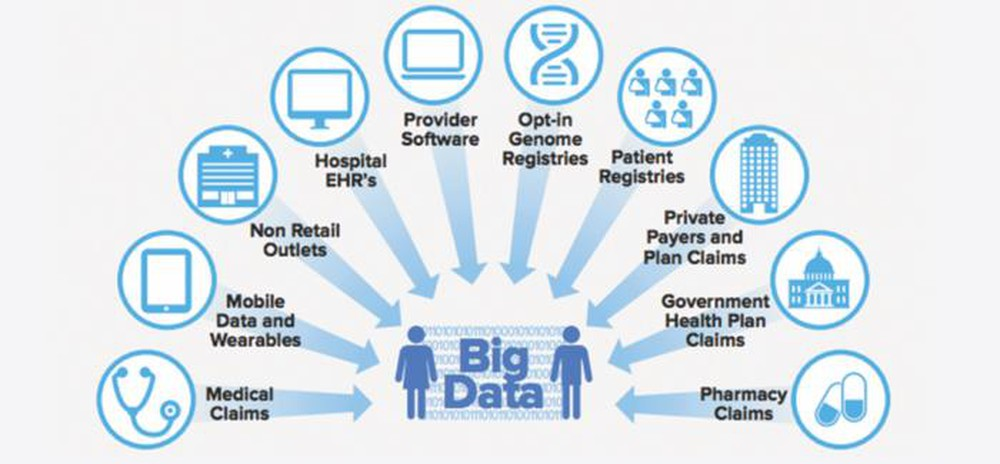
\includegraphics[scale=.3]{b-1.jpg}
	\caption{Ứng dụng của Big data}
\end{figure}
\section{NoSQL}
\subsubsection{Tổng quan về cơ sở dữ liệu NoSQL}
Khi làm việc với database, chúng ta đã quá quen với SQL Server, MySQL, PostgreSQL, Oracle,… Điểm chung của những database này là sử dụng ngôn ngữ SQL để truy vấn dữ liệu. Nhưng có 1 dạng database khác với những đặc tính khác biệt được gọi chung dưới cái tên là NoSQL. Thuật ngữ NoSQL được giới thiệu lần đầu vào năm 1998 sử dụng làm tên gọi chung cho các \textit{"lightweight open source relational database"} (cơ sở dữ liệu quan hệ mã nguồn mở nhỏ) nhưng không sử dụng SQL cho truy vấn. Thuật ngữ NoSQL đánh dấu bước phát triển của thế hệ database mới: \textit{distributed} (phân tán) + \textit{non-relational} (không ràng buộc), đây là 2 đặc tính quan trọng nhất. \\\\
Người ta phát triển NoSQL xuất phát từ yêu cầu cần những database có khả năng lưu trữ dữ liệu với lượng cực lớn, truy vấn dữ liệu với tốc độ cao mà không đòi hỏi quá nhiều về năng lực phần cứng cũng như tài nguyên hệ thống và tăng khả năng chịu lỗi. Đây là những vấn đề mà các relational database không thể giải quyết được. Lượng dữ liệu mà các hệ thống cần phải xử lý giờ đây ngày một lớn. Ví dụ như Google, Facebook phải lưu trữ và xử lý một lượng dữ liệu cực lớn mỗi ngày.
\subsubsection{Một số đặc điểm của NoSQL}
\begin{itemize}
	\item \textbf{High Scalability:} Gần như không có một giới hạn cho dữ liệu và người dùng trên hệ thống.
	\item \textbf{High Availability:}Do chấp nhận sự trùng lặp trong lưu trữ nên nếu một node (commodity machine) nào đó bị chết cũng không ảnh hưởng tới toàn bộ hệ thống.
	\item \textbf{Atomicity:}  Độc lập data state trong các operation.
	\item \textbf{Consistency:} chấp nhận tính nhất quán yếu, có thể không thấy ngay được sự thay đổi mặc dù đã cập nhật dữ liệu.
	\item \textbf{Durability:} dữ liệu có thể tồn tại trong bộ nhớ máy tính nhưng đồng thời cũng được lưu trữ lại đĩa cứng.
	\item \textbf{Deployment Flexibility:} việc bổ sung thêm/loại bỏ các node, hệ thống sẽ tự động nhận biết để lưu trữ mà không cần phải can thiệp bằng tay. Hệ thống cũng không đòi hỏi cấu hình phần cứng mạnh, đồng nhất.
	\item \textbf{Modeling flexibility: }  Key-Value pairs, Hierarchical data (dữ liệu cấu trúc), Graphs.
	\item \textbf{Query Flexibility:} Multi-Gets, Range queries (load một tập giá trị dựa vào một dãy các khóa). 
\end{itemize}
\chapter{Cơ sở dữ liệu phân tán}
\section{Các khái niệm cơ bản trong cơ sở dữ liệu phân tán}
\subsubsection{Cơ sở dữ liệu phân tán}
Một tuyển tập dữ liệu có quan hệ logic với nhau, được phân bố trên máy tính của một mạng máy tính. 
\subsubsection{Hệ quản trị CSDL phân tán} Hệ thống phần mềm cho phép quản lý CSDL phân tán và đảm bảo tính trong suốt về sự phân tán đối với người dùng.
\subsubsection{Ứng dụng cục bộ} Là ứng dụng được yêu cầu và thực hiện trên máy tính ở một nút trong hệ CSDL phân tán và chỉ liên quan đến CSDL tại nút đó.
\subsubsection{Ứng dụng toàn cục} Là ứng dụng được yêu câu truy nhập dữ liệu ở nhiều nút thông qua hệ thống truyền thông.
\section{Đánh giá cơ sở dữ liệu phân tán}
\subsection{Ưu điểm và nhược điểm của cơ sở dữ liệu phân tán}
\subsubsection{Ưu điểm}
\begin{itemize}
	\item Phù hợp với cấu trúc của tổ chức
	\item Nâng cao khả năng chia sẻ và tính tự trị địa phương
	\item Nâng cao tính sẵn sàng, tính tin cậy
	\item Nâng cao hiệu năng
	\item Dễ mở rộng, phát triển
\end{itemize}
\subsubsection{Nhược điểm}
\begin{itemize}
	\item Thiết kế cơ sở dữ liệu phức tạp hơn
	\item Khó điều chuyển tính nhất quán dữ liệu
	\item Khó phát hiện và xử lý lỗi
	\item Vấn đều bảo mật
	\item Giá thành cao
	\item Thiếu chuẩn mực
	\item Thiếu kinh nghiệm
\end{itemize}
\subsection{Một số vấn đề đối với cơ sở dữ liệu phân tán}
\subsubsection{Vấn đề về thiết kế}
\begin{itemize}
	\item Cách phân bố cơ sở dữ liệu?
	\item Vấn đề nhân bản dữ liệu
	\item Vấn đề liên quan trong thư mục quản lý
\end{itemize}
\subsubsection{Vấn đề xử lý truy vấn}
\begin{itemize}
	\item Chuyển các giao tác người dùng thành các chỉ thị thao tác trên dữ liệu
	\item Vấn đề tối ưu hóa
	\item Tối thiểu chi phí truyền dữ liệu và xử lý cục bộ
	\item Không có công thức chung
\end{itemize}
\subsubsection{Vấn đề điều khiển tương tranh}
\begin{itemize}
	\item Đồng bộ hóa các truy xuất tương tranh
	\item Tính nhất quán và tính riêng biệt của các giao tác
	\item Quản lý deadlock
\end{itemize}
\subsubsection{Vấn đề độ tin cậy}
\begin{itemize}
	\item Khả năng đáp ứng của hệ thống đối với các lỗi
\end{itemize}
\section{Xây dựng kiến trúc cơ sở dữ liệu phân tán}
Do sự đa dạng, không có kiến trúc nào được công nhận tương đương với kiến trúc 3 mức ANSI/SPARC. Một kiến trúc tham khảo bao gồm: 
\begin{itemize}
	\item Tập các sơ đồ ngoài toàn cục (Global external schema)
	\item Sơ đồ khái niệm toàn cục (Global conceptual schema)
	\item Sơ đồ phân đoạn (Fragmentation schema) và sơ đồ định vị (Allocation schema)
	\item Tập các sơ đồ cho mỗi hệ CSDL cục bộ tuân theo tiêu chuẩn 3 mức ANSI/SPARC
\end{itemize} 
\subsubsection{Sơ đồ tổng thể}
Sơ đồ này xác định tất cả các dữ liệu sẽ được lưu trữ trong CSDL phân tán. Sơ đồ tổng thể có thể được định nghĩa một cách chính xác theo cách như trong CSDL không phân tán. Ở đây sẽ sử dụng mô hình quan hệ để hình thành nên sơ đồ này. Sử dụng mô hình này, sơ đồ tổng thể bao gồm định nghĩa của một tập các quan hệ tổng thể. 
\subsubsection{Sơ đồ phân đoạn}
Mỗi quan hệ tổng thể có thể chia thành một vài phần nhỏ hơn không giao nhau được gọi là đoạn (fragments). Có nhiều cách khác nhau để thực hiện việc phân chia này. Sơ đồ tổng thể mô tả các ánh xạ giữa các quan hệ tổng thể và các đoạn được định nghĩa trong sơ đồ phân đoạn. Ánh xạ này là một- nhiều. Có thể có nhiều đoạn liên kết tới một quan hệ tổng thể, nhưng mỗi đoạn chỉ liên kết tới nhiều nhất là một quan hệ tổng thể. Các đoạn được chỉ ra bằng tên của quan hệ tổng thể cùng với tên của chỉ mục đoạn.
\subsubsection{Sơ đồ định vị} 
Các đoạn là các phần logic của một quan hệ tổng thể được định vị trên một hoặc nhiều vị trí vật lý trên mạng. Sơ đồ định vị xác định đoạn nào ở trạm nào. Lưu ý rằng, kiểu ánh xạ được định nghĩa trong sơ đồ định vị quyết định CSDL phân tán là dư thừa hay không. Tất cả các đoạn liên kết với cùng một quan hệ tổng thể $R$ và được định vị tại cùng một trạm $j$ cấu thành ảnh vật lý của quan hệ tổng thể $R$ tại trạm $j$. Bởi vậy, có thể ánh xạ một-một giữa một ảnh vật lý và một cặp (quan hệ tổng thể, trạm). Các ảnh vật lý có thể được chỉ ra bằng tên của một quan hệ tổng thể và một chỉ mục trạm. 
\subsubsection{Sơ đồ ánh xạ địa phương}
Ánh xạ các ảnh vật lý tới các đối tượng được các hệ quản trị CSDL địa phương thao tác tại các trạm. Ánh xạ này phụ thuộc vào các hệ quản trị CSDL địa phương.
\section{Thiết kế cơ sở dữ liệu phân tán}
\subsection{Kỹ thuật phân đoạn}
Phân hoạch cơ sở dữ liệu thành các đoạn (fragments): sự phân đoạn cho phép phân chia một đối tượng đơn lẻ thành hai hay nhiều mảnh. Thông tin phân đoạn được lưu trữ trong catalog dữ liệu phân tán. Phần mềm xử lý giao tác sẽ truy nhập thông tin ở đây để xử lý các yêu cầu của người dùng. Việc chia quan hệ tổng thể thành các đoạn có thể thực hiện bằng cách áp dụng các kiểu phân đoạn sau: 
\begin{itemize}
	\item Phân đoạn ngang: Dùng phép chọn để phân đoạn
	\item Phân đoạn dọc: Dùng phép chiếu để phân đoạn
	\item Phân đoạn hỗn hợp: Dùng cả phép chọn và phép chiếu để phân đoạn 
	\item Phân đoạn ngang suy diễn: Dùng phép nửa nối để phân đoạn
\end{itemize}
\subsection{Các ràng buộc trong thiết kế phân đoạn}
\subsubsection{Tính đầy đủ}
Toàn bộ dữ liệu của quan hệ tổng thể phải được ánh xạ vào các đoạn quan hệ và ngược lại. Điều này có nghĩa là, không tồn tại một mục dữ liệu nào thuộc vào quan hệ tổng thể mà không thuộc vào bất kỳ một đoạn nào. 
\subsubsection{Tính phục hồi}
Quan hệ tổng thể có thể được xây dựng lại từ các đoạn mà nó đã tách ra. Điều kiện này là hiển nhiên, bởi vì trong thực tế chỉ có các đoạn được lưu trữ trong CSDL phân tán, và quan hệ tổng thể phải được xây dựng lại thông qua các đoạn khi cần thiết.
\subsubsection{Tính tách biệt}
các đoạn được tách ra từ quan hệ tổng thể phải là rời nhau. Vì vậy, việc tạo các bản sao phải rõ ràng với các đoạn được chia. Tuy nhiên, điều kiện này chỉ áp dụng chính vào việc phân đoạn ngang, trong khi việc phân đoạn dọc nhiều khi vẫn được phép vi phạm điều kiện này.
\section{Tính trong suốt của cơ sở dữ liệu phân tán}
\subsection{Trong suốt phân đoạn (Fragmentation transparency)}
Trong suốt phân đoạn: là cấp độ cao nhất của mức độ trong suốt, người sử dụng hoặc chương 
trình ứng dụng chỉ làm việc trên các quan hệ của cơ sở dữ liệu. Khi dữ liệu đã được phân đoạn thì việc truy cập vào CSDL được thực hiện bình thường như là chưa bị phân tán và không ảnh hưởng tới người sử dụng. 
\subsection{Trong suốt về vị trí (Location transparency)}
Người sử dụng không cần biết về vị trí vật lý của dữ liệu mà có quyền truy cập đến cơ sở dữ liệu tại bất cứ vị trí nào. Các thao tác để lấy hoặc cập nhật một dữ liệu từ xa được tự động thực hiện bởi hệ thống tại điểm đưa ra yêu cầu. 
\subsection{Trong suốt ánh xạ địa phương (Local mapping transparency)}
Người dùng cuối hoặc người lập trình biết tên các đoạn và vị trí của các đoạn.
\subsection{Trong suốt nhân bản (Replication transparency)}
Mức trong suốt bản sao liên quan chặt chẽ tới mức trong suốt định vị. Mức trong suốt bản sao có nghĩa là người sử dụng không biết bản sao của đoạn đặt ở vị trí nào. Mức trong suốt bản sao tương đương mức trong suốt định vị. Tuy nhiên, trong những trường hợp thực tế người sử dụng không có mức trong suốt định vị nhưng lại có mức trong suốt bản sao.

\chapter{Hệ quản trị cơ sở dữ liệu Oracle}
\section{Lecture 1}
Hướng dẫn cài đặt hệ quản trị cơ sở dữ liệu Oracle.
\section{Lecture 2}
\subsection{Practice 1}
\begin{boxedminipage}[t]{15.5cm}
	Create the DEPT table based on the following table instance chart. Place the syntax in a script called lab\_09\_01.sql,
	then execute the statement in the script to create the table. Confirm that the table is created.
\end{boxedminipage}
\newline
\\
\textbf{Mã nguồn}
\\
\newline
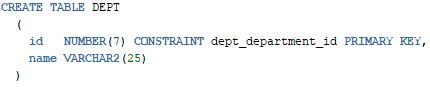
\includegraphics[scale=1]{p1.jpg}\\
\textbf{Kết quả}\\\\
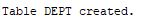
\includegraphics[scale=1]{kp1.jpg}

\subsection{Practice 2}
\begin{boxedminipage}[t]{15.5cm}
	Populate the DEPT table with data from the DEPARTMENTS table. Include only columns that you need.
\end{boxedminipage}
\newline
\\
\textbf{Mã nguồn}\\
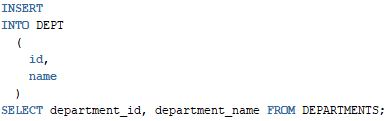
\includegraphics[scale=1]{p2.jpg}\\
\textbf{Kết quả}\\\\
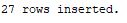
\includegraphics[scale=1]{kp2.jpg}

\subsection{Practice 3}
\begin{boxedminipage}[t]{15.5cm}
	Create the EMP table based on the following table instance chart. Place the syntax in a script called lab\_09\_03.sql, and then execute the statement in the script to create the table. Confirm that the table is created.
\end{boxedminipage}
\newline
\\
\textbf{Mã nguồn}\\\\
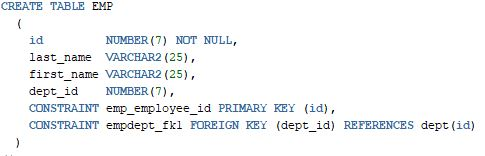
\includegraphics[scale=1]{p3.jpg}\\
\textbf{Kết quả}\\\\
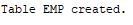
\includegraphics[scale=1]{kp3.jpg}

\subsection{Practice 4}
\begin{boxedminipage}[t]{15.5cm}
	Create the EMPLOYEES2 table based on the structure of the EMPLOYEES table. Include only the EMPLOYEE\_ID, FIRST\_NAME, LAST\_NAME, SALARY, and DEPARTMENT\_ID columns. Name the columns in your new table ID, FIRST\_NAME, LAST\_NAME, SALARY , and DEPT\_ID, respectively.
\end{boxedminipage}
\newline
\\
\textbf{Mã nguồn}\\\\
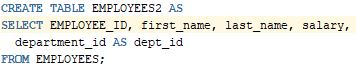
\includegraphics[scale=1]{p4.jpg}\\
\textbf{Kết quả}\\\\
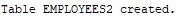
\includegraphics[scale=1]{kp4.jpg}

\subsection{Practice 5}
\begin{boxedminipage}[t]{4.5cm}
	Drop the EMP table.
\end{boxedminipage}
\newline
\\
\textbf{Mã nguồn}\\\\
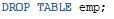
\includegraphics[scale=1]{p5.jpg}\\
\textbf{Kết quả}\\\\
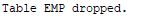
\includegraphics[scale=1]{kp5.jpg}

\subsection{Practice 6}
\begin{boxedminipage}[t]{14.5cm}
Create a nonunique index on the DEPT\_ID column in the DEPT table.
\end{boxedminipage}
\newline
\\
\textbf{Mã nguồn}\\\\
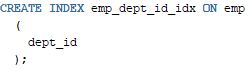
\includegraphics[scale=1]{p6.jpg}

\section{Lecture 3}
\subsection{Practice 1}
\begin{boxedminipage}[t]{15.5cm}
	The staff in the HR department wants to hide some of the data in the EMPLOYEES table.They want a view called EMPLOYEES\_VU based on the employee numbers, employee names, and department numbers from the EMPLOYEES table. They want the heading for the employee name to be EMPLOYEE.
\end{boxedminipage}
\newline
\\
\textbf{Mã nguồn}
\\
\newline
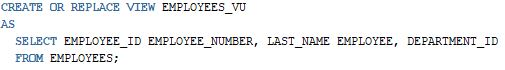
\includegraphics[scale=1]{p13.jpg}\\
\textbf{Kết quả}\\\\
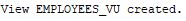
\includegraphics[scale=1]{kp13.jpg}

\subsection{Practice 2}
\begin{boxedminipage}[t]{15.5cm}
	Confirm that the view works. Display the contents of the EMPLOYEES\_VU view.
\end{boxedminipage}
\newline
\\
\textbf{Mã nguồn}
\\
\newline
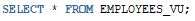
\includegraphics[scale=1]{p23.jpg}\\
\textbf{Kết quả}\\\\
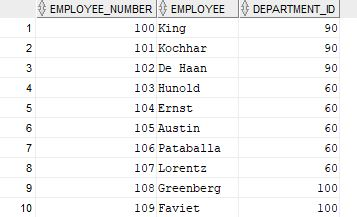
\includegraphics[scale=1]{kp23.jpg}

\subsection{Practice 3}
\begin{boxedminipage}[t]{15.5cm}
	Using your EMPLOYEES\_VU view, write a query for the HR department to display all employee names and department numbers.
\end{boxedminipage}
\newline
\\
\textbf{Mã nguồn}
\\
\newline
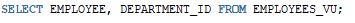
\includegraphics[scale=1]{p33.jpg}\\
\textbf{Kết quả}\\\\
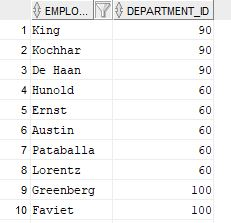
\includegraphics[scale=1]{kp33.jpg}

\subsection{Practice 4}
\begin{boxedminipage}[t]{15.5cm}
Department 50 needs access to its employee data. Create a view named DEPT50 that contains 
the employee numbers, employee last names, and department numbers for all employees in department 50. \\
You have been asked to label the view columns EMPNO, EMPLOYEE, and DEPTNO. For security purposes, do not allow an employee to be reassigned to another department through the view.\\
* Display the structure and contents of the DEPT50 view.\\
* Test your view. Attempt to reassign Mohammed to department 80.
\end{boxedminipage}
\newline
\\
\textbf{Mã nguồn}
\\
\newline
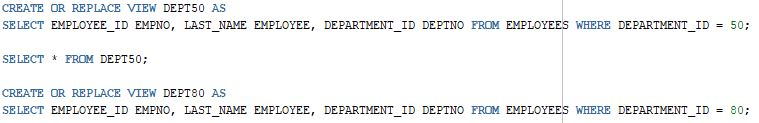
\includegraphics[scale=.78]{p43.jpg}\\
\textbf{Kết quả}\\\\
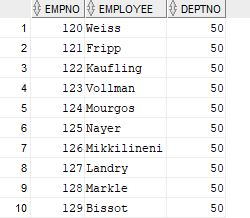
\includegraphics[scale=1]{kp43.jpg}\\
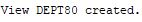
\includegraphics[scale=1]{kp432.jpg}


\subsection{Practice 5}
\begin{boxedminipage}[t]{15.5cm}
* You need a sequence that can be used with the primary key column of the DEPT table. 
The sequence should start at 200 and have a maximum value of 1,000. Have your sequence increment by 10. Name the sequence DEPT\_ID\_SEQ.\\ * To test your sequence, write a script to insert two rows in the DEPT table. 
Be sure to use the sequence that you created for the ID column. Add two departments: Education and Administration. 
Confirm your additions. Run the commands in your script.
\end{boxedminipage}
\newline
\\
\textbf{Mã nguồn}
\\
\newline
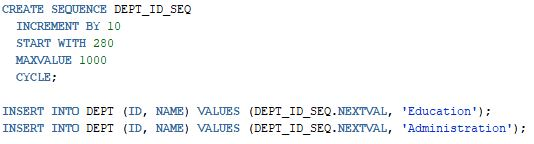
\includegraphics[scale=1]{p53.jpg}\\
\textbf{Kết quả}\\\\
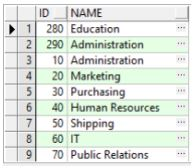
\includegraphics[scale=.9]{kp53.jpg}

\subsection{Practice 6}
\begin{boxedminipage}[t]{12.5cm}
	Create a synonym for your EMPLOYEES table. Call it EMP.
\end{boxedminipage}
\newline
\\
\textbf{Mã nguồn}
\\
\newline
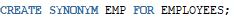
\includegraphics[scale=1]{p63.jpg}

\section{Lecture 4}
\subsection{Practice 1,2}
\begin{boxedminipage}[t]{3cm}
	True or False?
\end{boxedminipage}\\
\newline
\textbf{Kết quả} \qquad
\textbf{1. True \qquad 2. False}

\subsection{Practice 3}
\begin{boxedminipage}[t]{15.5cm}
	There are four coding errors in the following statement. Can you identify them?
\end{boxedminipage}
\newline
\\
\textbf{Mã nguồn}
\\
\newline
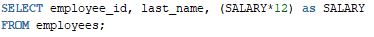
\includegraphics[scale=1]{34.jpg}\\
\textbf{Kết quả}\\\\
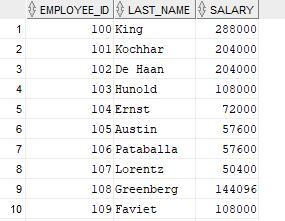
\includegraphics[scale=1]{k34.jpg}

\subsection{Practice 4}
\begin{boxedminipage}[t]{15.5cm}
	The HR department needs a query to display all unique job codes from the EMPLOYEES table.
\end{boxedminipage}
\newline
\\
\textbf{Mã nguồn}
\\
\newline
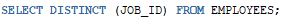
\includegraphics[scale=1]{44.jpg}\\
\textbf{Kết quả}\\\\
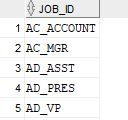
\includegraphics[scale=1]{k44.jpg}

\subsection{Practice 5}
\begin{boxedminipage}[t]{15.5cm}
	The HR department has requested a report of all employees and their job IDs. 
	Display the last name concatenated with the job ID (separated by a comma and space) 
	and name the column Employee and Title.
\end{boxedminipage}
\newline
\\
\textbf{Mã nguồn}
\\
\newline
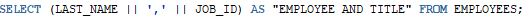
\includegraphics[scale=1]{54.jpg}\\
\textbf{Kết quả}\\\\
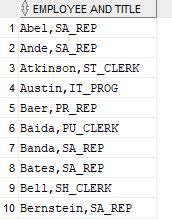
\includegraphics[scale=1]{k54.jpg}

\subsection{Practice 6}
\begin{boxedminipage}[t]{15.5cm}
	The HR departments needs to find high-salary and low-salary employees. 
	Display the last name and salary of employees who earn between 5,000\$ and 12,000\$ and are in department 20 or 50. Label the columns Employee and Monthly Salary, respectively.
\end{boxedminipage}
\newline
\\
\textbf{Mã nguồn}
\\
\newline
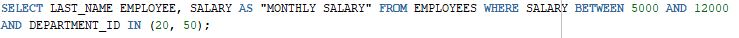
\includegraphics[scale=.8]{64.jpg}\\
\textbf{Kết quả}\\\\
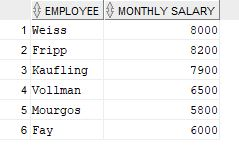
\includegraphics[scale=1]{k64.jpg}

\subsection{Practice 7}
\begin{boxedminipage}[t]{15.5cm}
	Create a report to display the last name, salary, and commission of all employees who earn commissions. 
	Sort data in descending order of salary and commissions.
\end{boxedminipage}
\newline
\\
\textbf{Mã nguồn}
\\
\newline
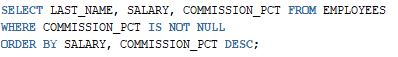
\includegraphics[scale=1]{74.jpg}\\
\textbf{Kết quả}\\\\
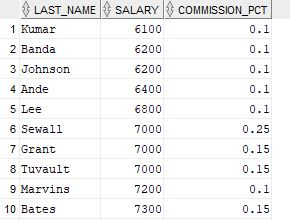
\includegraphics[scale=1]{k74.jpg}

\subsection{Practice 8}
\begin{boxedminipage}[t]{15.5cm}
	Display the last name of all employees who have both an a and an e in their last name.
\end{boxedminipage}
\newline
\\
\textbf{Mã nguồn}
\\
\newline
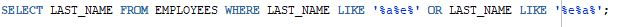
\includegraphics[scale=.95]{84.jpg}\\
\textbf{Kết quả}\\\\
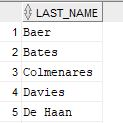
\includegraphics[scale=1]{k84.jpg}

\subsection{Practice 9}
\begin{boxedminipage}[t]{15.5cm}
	Display the last name, job, and salary for all employees whose job is SA\_REP or ST\_CLERK and 
	whose salary is not equal to \$2,500, \$3,500, or \$7,000.
\end{boxedminipage}
\newline
\\
\textbf{Mã nguồn}
\\
\newline
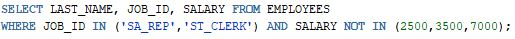
\includegraphics[scale=1]{94.jpg}\\
\textbf{Kết quả}\\\\
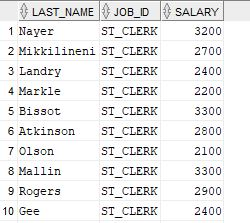
\includegraphics[scale=1]{k94.jpg}

\section{Lecture 5}
\subsection{Practice 1}
\begin{boxedminipage}[t]{15.5cm}
	Write a query that displays the last name (with the first letter uppercase and all other letters lowercase) 
	and the length of the last name for all employees whose name starts with the letters J, A, or M. 
	Give each column an appropriate label. Sort the results by the employees’ last names.
\end{boxedminipage}
\newline
\\
\textbf{Mã nguồn}
\\
\newline
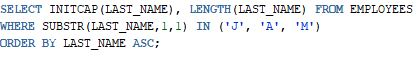
\includegraphics[scale=1]{15.jpg}\\
\textbf{Kết quả}\\\\
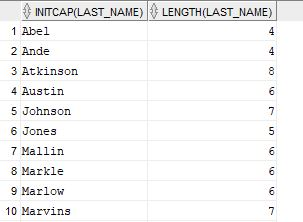
\includegraphics[scale=1]{k15.jpg}

\subsection{Practice 2}
\begin{boxedminipage}[t]{15.5cm}
The HR department wants to find the length of employment for each employee. 
For each employee, display the last name and calculate the number of months between today and the date 
on which the employee was hired. Label the column MONTHS\_WORKED. Order your results by the number 
of months employed. Round the number of months up to the closest whole number.
\end{boxedminipage}
\newline
\\
\textbf{Mã nguồn}
\\
\newline
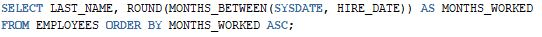
\includegraphics[scale=1]{25.jpg}\\
\textbf{Kết quả}\\\\
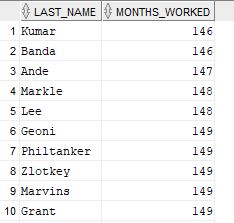
\includegraphics[scale=1]{k25.jpg}

\subsection{Practice 3}
\begin{boxedminipage}[t]{15.5cm}
	Display each employee’s last name, hire date, and salary review date, 
	which is the first Monday after six months of service. Label the column REVIEW. 
	Format the dates to appear in the format similar to “Monday, the Thirty-First of July, 2000.”
\end{boxedminipage}
\newline
\\
\textbf{Mã nguồn}
\\
\newline
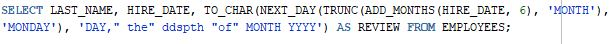
\includegraphics[scale=.95]{35.jpg}\\
\textbf{Kết quả}\\\\
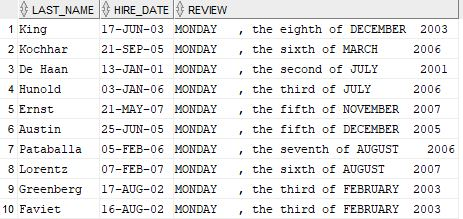
\includegraphics[scale=1]{k35.jpg}

\subsection{Practice 4}
\begin{boxedminipage}[t]{15.5cm}
Create a query that displays the employees’ last names and commission amounts. 
If an employee does not earn commission, show “No Commission.” Label the column COMM.
\end{boxedminipage}
\newline
\\
\textbf{Mã nguồn}
\\
\newline
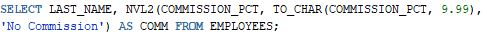
\includegraphics[scale=1]{45.jpg}\\
\textbf{Kết quả}\\\\
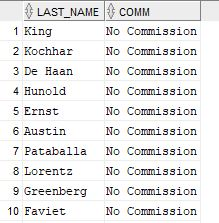
\includegraphics[scale=1]{k45.jpg}

\subsection{Practice 5}
\begin{boxedminipage}[t]{15.5cm}
	Using the DECODE function, write a query that displays the grade of all employees
	based on the value of the column JOB\_ID, using the following data:
	\begin{center}
	\begin{tabular}{|l|c|}
		\hline
		JOB & GRADE \\
		\hline
		AD\_PRES & A \\
		\hline
		ST\_MAN & B \\
		\hline
		IT\_PROG & C \\
		\hline
		SA\_REP & D \\
		\hline
		ST\_CLERK & E \\
		\hline
	\end{tabular}
	\end{center}
	None of the above 0
\end{boxedminipage}
\newline
\\
\textbf{Mã nguồn}
\\
\newline
\includegraphics[scale=1]{55.jpg}\\
\textbf{Kết quả}\\\\
\includegraphics[scale=1]{k55.jpg}

\subsection{Practice 6}
\begin{boxedminipage}[t]{15.5cm}
	Rewrite the query so that the user is prompted to enter a letter that starts the last name. 
	For example, if the user enters H when prompted for a letter, then the output should show all 
	employees whose last name starts with the letter H.
\end{boxedminipage}
\newline
\\
\textbf{Mã nguồn}
\\
\newline
\includegraphics[scale=1]{65.jpg}\\
\textbf{Kết quả}\\\\
\includegraphics[scale=1]{k65.jpg}

\subsection{Practice 7}
\begin{boxedminipage}[t]{15.5cm}
Find the highest, lowest, sum, and average salary of all employees. 
Label the columns Maximum, Minimum, Sum, and Average, respectively. 
Round your results to the nearest whole number..
\end{boxedminipage}
\newline
\\
\textbf{Mã nguồn}
\\
\newline
\includegraphics[scale=1]{75.jpg}\\
\textbf{Kết quả}\\\\
\includegraphics[scale=1]{k75.jpg}

\subsection{Practice 8}
\begin{boxedminipage}[t]{15.5cm}
	Modify the query in Exercise 1 to display the minimum, maximum, sum, and average salary for each job type.
\end{boxedminipage}
\newline
\\
\textbf{Mã nguồn}
\\
\newline
\includegraphics[scale=1]{85.jpg}\\
\textbf{Kết quả}\\\\
\includegraphics[scale=1]{k85.jpg}

\subsection{Practice 9}
\begin{boxedminipage}[t]{15.5cm}
	 Determine the number of managers without listing them. Label the column Number of Managers. 
	Hint: Use the MANAGER\_ID column to determine the number of managers.
\end{boxedminipage}
\newline
\\
\textbf{Mã nguồn}
\\
\newline
\includegraphics[scale=1]{95.jpg}\\
\textbf{Kết quả}\\\\
\includegraphics[scale=1]{k95.jpg}

\subsection{Practice 10}
\begin{boxedminipage}[t]{15.5cm}
Create a report to display the manager number and the salary of the lowest-paid employee for that manager. 
Exclude anyone whose manager is not known. Exclude any groups where the minimum salary is \$6,000 or less. 
Sort the output in descending order of salary.
\end{boxedminipage}
\newline
\\
\textbf{Mã nguồn}
\\
\newline
\includegraphics[scale=1]{105.jpg}\\
\textbf{Kết quả}\\\\
\includegraphics[scale=1]{k105.jpg}

\section{Lecture 6}
\subsection{Practice 1}
\begin{boxedminipage}[t]{15.5cm}
	The HR department needs a report of all employees. Write a query to display the last name, 
	department number, and department name for all employees.
\end{boxedminipage}
\newline
\\
\textbf{Mã nguồn}
\\
\newline
\includegraphics[scale=1]{16.jpg}\\
\textbf{Kết quả}\\\\
\includegraphics[scale=1]{k16.jpg}

\subsection{Practice 2}
\begin{boxedminipage}[t]{15.5cm}
	(A) Create a report to display employees’ last name and employee number along with 
	their manager’s last name and manager number. Label the columns Employee, Emp\#, Manager, and Mgr\#, respectively.\\
	(B) Modify Part A to display all employees including King, who has no manager. Order the results by the employee number.
\end{boxedminipage}
\newline
\\
\textbf{Mã nguồn}
\\
\newline
\includegraphics[scale=1]{26a.jpg}\\
\includegraphics[scale=1]{26b.jpg}\\
\textbf{Kết quả}\\\\
\includegraphics[scale=1]{k26a.jpg}\\
\includegraphics[scale=1]{k26b.jpg}

\subsection{Practice 3}
\begin{boxedminipage}[t]{15.5cm}
	The HR department needs to find the names and hire dates for all employees 
	who were hired before their managers, along with their managers’ names and hire dates.
\end{boxedminipage}
\newline
\\
\textbf{Mã nguồn}
\\
\newline
\includegraphics[scale=1]{36.jpg}\\
\textbf{Kết quả}\\\\
\includegraphics[scale=1]{k36.jpg}

\subsection{Practice 4}
\begin{boxedminipage}[t]{15.5cm}
	Display the employee number, last name, and salary of all employees who earn more than the average salary and 
	who work in a department with any employee whose last name contains a u.
\end{boxedminipage}
\newline
\\
\textbf{Mã nguồn}
\\
\newline
\includegraphics[scale=1]{46.jpg}\\
\textbf{Kết quả}\\\\
\includegraphics[scale=1]{k46.jpg}


\subsection{Practice 5}
\begin{boxedminipage}[t]{15.5cm}
The HR department needs a report with the following specifications:\\
- Last name and department ID of all the employees from the EMPLOYEES table, 
regardless of whether or not they belong to a department\\
- Department ID and department name of all the departments from the DEPARTMENTS table, 
regardless of whether or not they have employees working in them
Write a compound query to accomplish this .
\end{boxedminipage}
\newline
\\
\textbf{Mã nguồn}
\\
\newline
\includegraphics[scale=1]{56.jpg}\\
\textbf{Kết quả}\\\\
\includegraphics[scale=1]{k56.jpg}

\subsection{Practice 6}
\begin{boxedminipage}[t]{15.5cm}
	Create a report that lists the employee IDs and job IDs of those employees 
	who currently have a job title that is the same as their job title when they were 
	initially hired by the company (that is, they changed jobs but have now gone back 
	to doing their original job).
\end{boxedminipage}
\newline
\\
\textbf{Mã nguồn}
\\
\newline
\includegraphics[scale=1]{66.jpg}\\
\textbf{Kết quả}\\\\
\includegraphics[scale=1]{k66.jpg}

\subsection{Practice 7}
\begin{boxedminipage}[t]{15.5cm}
	The HR department needs a list of countries that have no departments located in them. 
	Display the country ID and the name of the countries. Use set operators to create this report.
\end{boxedminipage}
\newline
\\
\textbf{Mã nguồn}
\\
\newline
\includegraphics[scale=1]{76.jpg}\\
\textbf{Kết quả}\\\\
\includegraphics[scale=1]{k76.jpg}

\section{Lecture 7}
Không có bài tập.

\section{Lecture 8}
\subsection{Practice 1}
\begin{boxedminipage}[t]{15.5cm}
Write a query to display the following for those employees whose manager ID is less than 120:\\
- Manager ID\\
- Job ID and total salary for every job ID for employees who report to the same
manager\\
- Total salary of those managers
Total salary of those managers, irrespective of the job IDs

\end{boxedminipage}
\newline
\\
\textbf{Mã nguồn}
\\
\newline
\includegraphics[scale=1]{18.jpg}\\
\textbf{Kết quả}\\\\
\includegraphics[scale=1]{k18.jpg}


\subsection{Practice 2}
\begin{boxedminipage}[t]{15.5cm}
Observe the output from question 1. Write a query using the GROUPING function to determine whether the NULL values in the columns corresponding to the GROUP BY expressions are caused by the ROLLUP operation.

\end{boxedminipage}
\newline
\\
\textbf{Mã nguồn}
\\
\newline
\includegraphics[scale=1]{28.jpg}\\
\textbf{Kết quả}\\\\
\includegraphics[scale=1]{k28.jpg}

\subsection{Practice 3}
\begin{boxedminipage}[t]{15.5cm}
	Write a query to display the following for those employees whose manager ID is less than 120:\\
	- Manager ID\\
	- Job and total salaries for every job for employees who report to the same manager\\
	- Total salary of those managers\\
	- Cross-tabulation values to display the total salary for every job, irrespective of the manager \\
	- Total salary irrespective of all job titles
	
	
\end{boxedminipage}
\newline
\\
\textbf{Mã nguồn}
\\
\newline
\includegraphics[scale=1]{38.jpg}\\
\textbf{Kết quả}\\\\
\includegraphics[scale=1]{k38.jpg}

\subsection{Practice 4}
\begin{boxedminipage}[t]{15.5cm}
	Using GROUPING SETS, write a query to display the following groupings:\\
	- department\_id, manager\_id, job\_id\\
	- department\_id, job\_id\\
	- manager\_id, job\_id\\
	The query should calculate the sum of the salaries for each of these groups.
	
	
\end{boxedminipage}
\newline
\\
\textbf{Mã nguồn}
\\
\newline
\includegraphics[scale=1]{48.jpg}\\
\textbf{Kết quả}\\\\
\includegraphics[scale=1]{k48.jpg}

\section{Lecture 9, 10}
Không có bài tập.

\section{Lecture 11}
\subsection{Practice 1}
\begin{boxedminipage}[t]{9.5cm}
	Print last names, salaries, and department IDs.
	
	
\end{boxedminipage}
\newline
\\
\textbf{Mã nguồn}
\\
\newline
\includegraphics[scale=1]{111.jpg}\\
\textbf{Kết quả}\\\\
\includegraphics[scale=1]{k111.jpg}

\subsection{Practice 2}
\begin{boxedminipage}[t]{15.5cm}
Create a report that shows the hierarchy of the managers for the employee Lorentz.\\
* Don’t display Lorentz\\
* Display his immediate manager first.
\end{boxedminipage}
\newline
\\
\textbf{Mã nguồn}
\\
\newline
\includegraphics[scale=1]{211.jpg}\\
\textbf{Kết quả}\\\\
\includegraphics[scale=1]{k211.jpg}

\subsection{Practice 3}
\begin{boxedminipage}[t]{15.5cm}
	Produce a company organization chart that shows the management hierarchy. 
	Print the employee’s last name, employee ID, manager ID, and job ID.
	
	
	
\end{boxedminipage}
\newline
\\
\textbf{Mã nguồn}
\\
\newline
\includegraphics[scale=1]{311.jpg}\\
\textbf{Kết quả}\\\\
\includegraphics[scale=1]{k311.jpg}

\chapter{Bài tập kết thúc môn}
\section{Bài 1}
\begin{boxedminipage}[t]{15.5cm}
Kiểm tra 1 sinh viên đã đủ điều kiện tốt nghiệp chưa biết rằng các điều kiện để một sinh viên tốt nghiệp là:
\begin{itemize}
	\item Tích luỹ đủ số tín chỉ
	\item Điểm phẩy tốt nghiệp không nhỏ hơn 1.0, biết bảng đổi điểm như sau:	
\end{itemize}	
		\begin{center}
		\includegraphics[scale=.7]{bang.jpg}
		
	\end{center}
\end{boxedminipage}
\subsection{Mã nguồn Oracle}
\subsubsection{Bước 1: Tạo VIEW đổi điểm chữ sang điểm số.} 
\includegraphics[scale=1]{b1v1.jpg}
\subsubsection{Bước 2: Tạo VIEW lấy ra điểm số cao nhất của sinh viên} 
\includegraphics[scale=1]{b1v2.jpg}
\subsubsection{Bước 3: Tạo VIEW chứa tín chỉ tương ứng} 
\includegraphics[scale=1]{b1v3.jpg}
\subsubsection{Bước 4: Tạo VIEW lấy ra tổng số tín chỉ} 
\includegraphics[scale=1]{b1v2.jpg}
\subsubsection{Bước 5: Tạo thủ tục kiểm tra điều kiện tốt nghiệp của sinh viên} 
\includegraphics[scale=1]{b1o.jpg}
\subsubsection{Kết quả thực thi Oracle với ID = 1000}
\includegraphics[scale=1]{kb1o.jpg}

\subsection{Mã nguồn SQL}
Xây dựng các VIEW và thủ tục tương tự như Oracle.\\\\
\includegraphics[scale=1]{b1s1.jpg}\\
\includegraphics[scale=1]{b1s2.jpg}\\
\includegraphics[scale=.9]{bts3.jpg}
\subsubsection{Kết quả}
\includegraphics[scale=1]{b1s.jpg}\\
\subsection{Bình luận}
Trong Bước 1 Oracle, ta có thể thay hàm Decode bằng Case - When. Việc tạo VIEW cho ta những thuận lợi trong việc tính toán và đưa ra kết quả. Sự khác biệt của SQL và Oracle ở đây là trong SQL không có hàm Decode.

\section{Bài 2}
\begin{boxedminipage}[t]{15.5cm}
Viết thủ tục SP\_LOC\_DU\_LIEU cho phép nhập vào tên trường bất kỳ và một giá trị của trường (Ví dụ: SP\_LOC\_DU\_LIEU ‘dept\_name’, ‘Physics’). Kết quả trả về là dữ liệu sau khi lọc theo giá trị của trường dữ liệu đó. 	
\end{boxedminipage}

\subsection{Mã nguồn Oracle}
\subsubsection{Bước 1}
\includegraphics[scale=.85]{b2o1.jpg}
\subsubsection{Bước 2}
\includegraphics[scale=.85]{b2o2.jpg}
\subsubsection{Kết quả thực thi}
\includegraphics[scale=.57]{kb2o.jpg}\\

\subsection{Mã nguồn SQL}
\includegraphics[scale=.9]{b2s1.jpg}
\subsubsection{Bước 2}
\includegraphics[scale=.9]{b2s2.jpg}
\subsubsection{Kết quả thực thi}
\includegraphics[scale=.58]{kb2s.jpg}\\

\subsection{Bình luận}
Bằng cách tạo VIEW chứa tất cả các trường theo yêu cầu của đề bài, chúng ta có thể dễ dàng tạo thủ tục lọc dữ liệu với đầu vào là tên trường và giá trị tương ứng.
\section{Bài 3}
\begin{boxedminipage}[t]{15.5cm}
Viết thủ tục SP\_LOC\_DU\_LIEU cho phép nhập vào một biến kiểu table gồm 2 trường: tên trường và một giá trị của trường. Kết quả trả về là dữ liệu sau khi lọc theo danh sách các giá trị của các trường dữ liệu đó.	
\end{boxedminipage}

\subsection{Mã nguồn Oracle}
\subsubsection{Bước 1}
\includegraphics[scale=1]{b3o1.jpg}
\subsubsection{Bước 2}
\includegraphics[scale=.92]{b3o2.jpg}
\subsubsection{Kết quả thực thi}
\includegraphics[scale=1]{rb3o.jpg}\\\\
\includegraphics[scale=.55]{kb3o.jpg}
\subsection{Mã nguồn SQL}
\includegraphics[scale=.9]{b3s1.jpg}\\\\
\includegraphics[scale=.9]{b3s2.jpg}
\subsubsection{Kết quả thực thi}
\includegraphics[scale=.7]{kb3s.jpg}
\subsection{Bình luận}
Sử dụng kiểu dữ liệu TYPE OBJECT để lưu giữ các giá trị đầu vào rồi tiến hành lọc tương tự như bài 2.
\section{Bài 4}
\begin{boxedminipage}[t]{15.5cm}
	Sinh viên $A$ muốn học môn ‘Mobile Computing’ hỏi $A$ cần phải học qua những môn gì?	
\end{boxedminipage}

\subsection{Mã nguồn Oracle}

\subsection{Mã nguồn SQL}

\subsection{Bình luận}

\section{Bài 2}
\begin{boxedminipage}[t]{15.5cm}
	Viết thủ tục SP\_LOC\_DU\_LIEU cho phép nhập vào tên trường bất kỳ và một giá trị của trường (Ví dụ: SP\_LOC\_DU\_LIEU ‘dept\_name’, ‘Physics’). Kết quả trả về là dữ liệu sau khi lọc theo giá trị của trường dữ liệu đó. 	
\end{boxedminipage}

\subsection{Mã nguồn Oracle}

\subsection{Mã nguồn SQL}

\subsection{Bình luận}

\section{Bài 2}
\begin{boxedminipage}[t]{15.5cm}
	Viết thủ tục SP\_LOC\_DU\_LIEU cho phép nhập vào tên trường bất kỳ và một giá trị của trường (Ví dụ: SP\_LOC\_DU\_LIEU ‘dept\_name’, ‘Physics’). Kết quả trả về là dữ liệu sau khi lọc theo giá trị của trường dữ liệu đó. 	
\end{boxedminipage}

\subsection{Mã nguồn Oracle}

\subsection{Mã nguồn SQL}

\subsection{Bình luận}

\section{Bài 2}
\begin{boxedminipage}[t]{15.5cm}
	Viết thủ tục SP\_LOC\_DU\_LIEU cho phép nhập vào tên trường bất kỳ và một giá trị của trường (Ví dụ: SP\_LOC\_DU\_LIEU ‘dept\_name’, ‘Physics’). Kết quả trả về là dữ liệu sau khi lọc theo giá trị của trường dữ liệu đó. 	
\end{boxedminipage}

\subsection{Mã nguồn Oracle}

\subsection{Mã nguồn SQL}

\subsection{Bình luận}

\section{Bài 2}
\begin{boxedminipage}[t]{15.5cm}
	Viết thủ tục SP\_LOC\_DU\_LIEU cho phép nhập vào tên trường bất kỳ và một giá trị của trường (Ví dụ: SP\_LOC\_DU\_LIEU ‘dept\_name’, ‘Physics’). Kết quả trả về là dữ liệu sau khi lọc theo giá trị của trường dữ liệu đó. 	
\end{boxedminipage}

\subsection{Mã nguồn Oracle}

\subsection{Mã nguồn SQL}

\subsection{Bình luận}

\section{Bài 2}
\begin{boxedminipage}[t]{15.5cm}
	Viết thủ tục SP\_LOC\_DU\_LIEU cho phép nhập vào tên trường bất kỳ và một giá trị của trường (Ví dụ: SP\_LOC\_DU\_LIEU ‘dept\_name’, ‘Physics’). Kết quả trả về là dữ liệu sau khi lọc theo giá trị của trường dữ liệu đó. 	
\end{boxedminipage}

\subsection{Mã nguồn Oracle}

\subsection{Mã nguồn SQL}

\subsection{Bình luận}

\section{Bài 2}
\begin{boxedminipage}[t]{15.5cm}
	Viết thủ tục SP\_LOC\_DU\_LIEU cho phép nhập vào tên trường bất kỳ và một giá trị của trường (Ví dụ: SP\_LOC\_DU\_LIEU ‘dept\_name’, ‘Physics’). Kết quả trả về là dữ liệu sau khi lọc theo giá trị của trường dữ liệu đó. 	
\end{boxedminipage}

\subsection{Mã nguồn Oracle}

\subsection{Mã nguồn SQL}

\subsection{Bình luận}
\end{document}